\section{Neutrinos, Backgrounds, and Routing}

A valid reconstruction requires all packets to be collected regardless of neutrino type, energy within the valid range, interaction vertex, and should also be able to accept a range of incoming momentum angles.

\subsection{Combining the Digital and Physical Simulations}



%%% Example of Digital Simulation Reconstruction
\begin{figure*}
  \centering
  \begin{subfigure}[b]{0.475\textwidth}
      \centering
      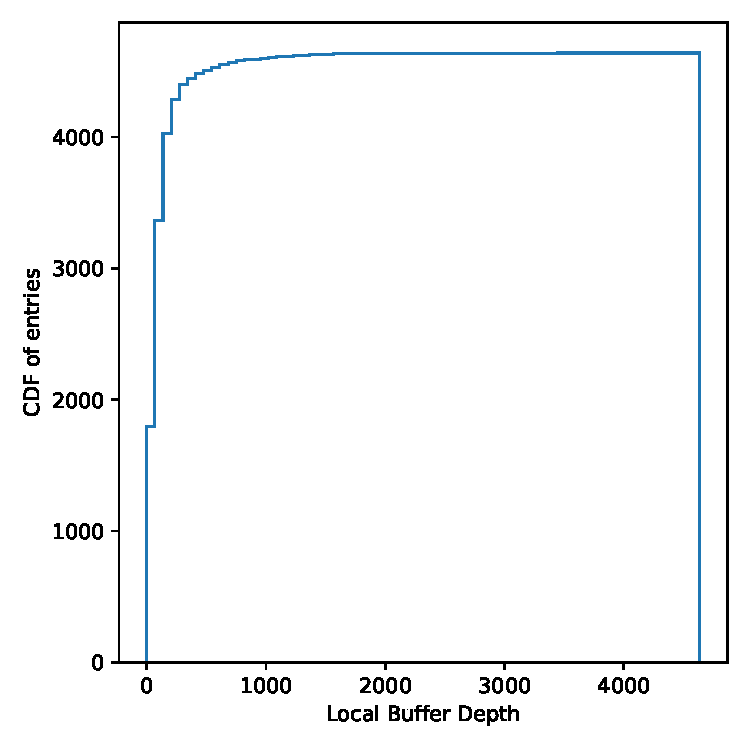
\includegraphics[width=\textwidth]{./images/mp60_16_slow_local_stack.pdf}
      \caption[Network2]%
      {{\small Network 1}}    
  \end{subfigure}
  \hfill
  \begin{subfigure}[b]{0.475\textwidth}  
      \centering 
      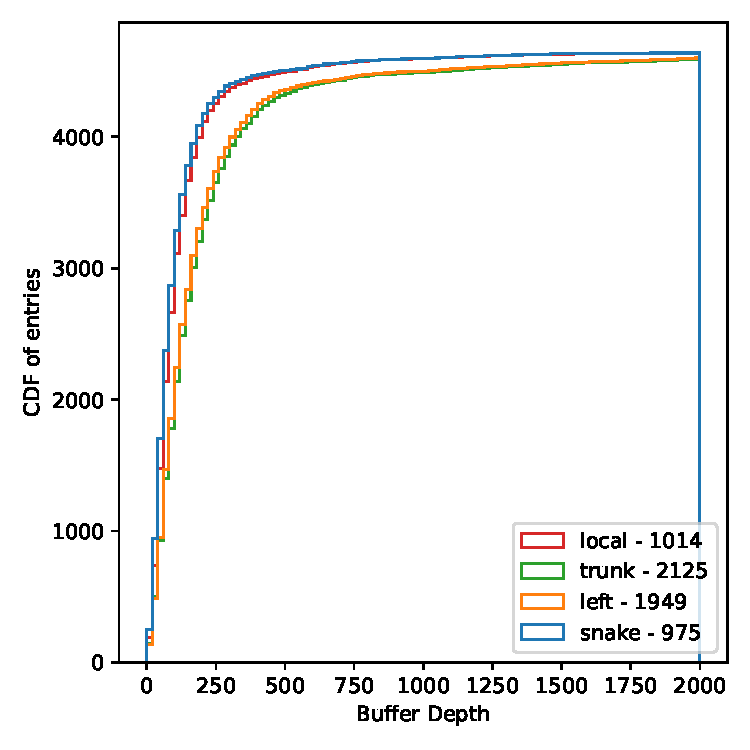
\includegraphics[width=\textwidth]{./images/mp60_16_slow_remote_stack.pdf}
      \caption[]%
      {{\small remote stack}}    
  \end{subfigure}
  \vskip\baselineskip
  \begin{subfigure}[b]{0.475\textwidth}   
      \centering 
      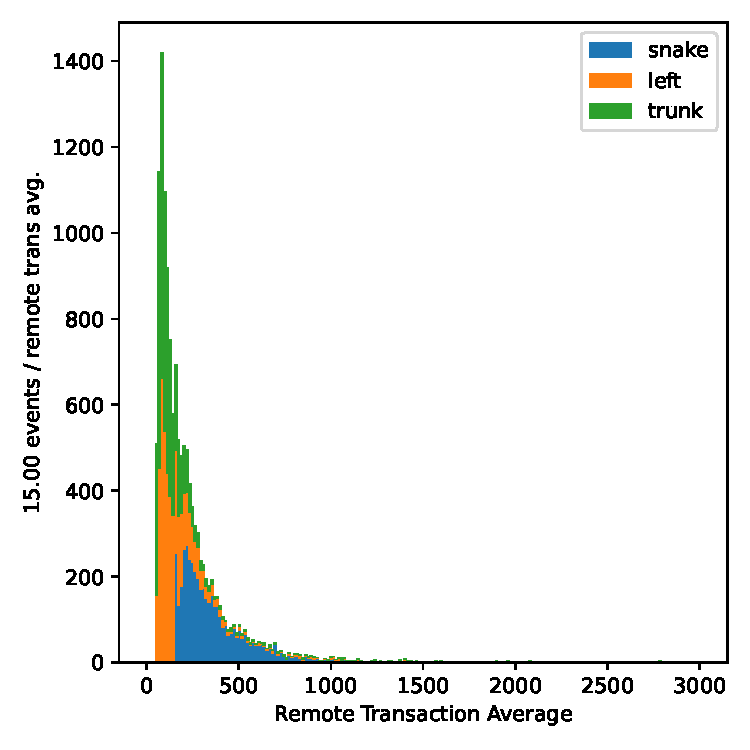
\includegraphics[width=\textwidth]{./images/mp60_16_slow_remote_transactions.pdf}
      \caption[]%
      {{\small transact}}    
  \end{subfigure}
  \hfill
  \begin{subfigure}[b]{0.475\textwidth}   
      \centering 
      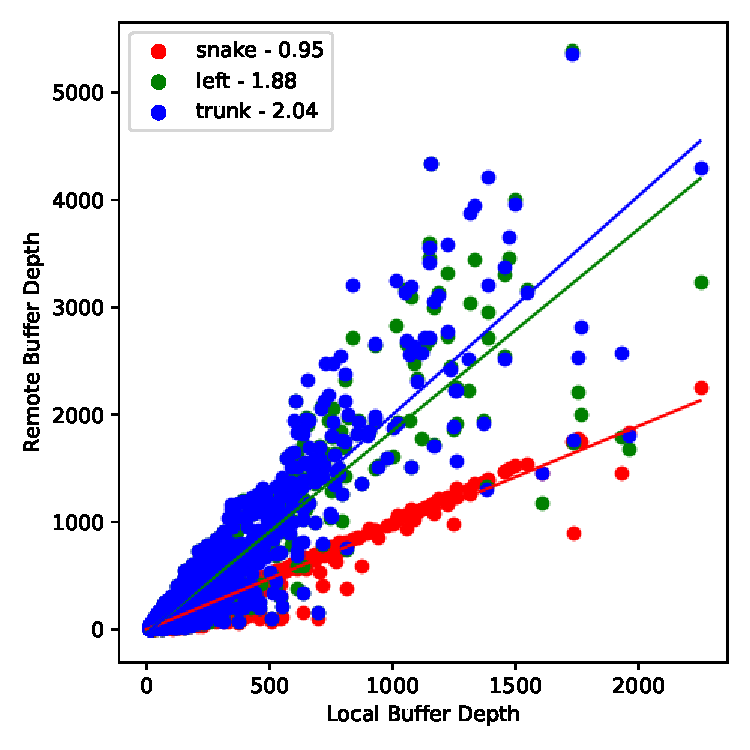
\includegraphics[width=\textwidth]{./images/mp60_16_slow_route_fits.pdf}
      \caption[]%
      {{\small route fits}}    
  \end{subfigure}
  \caption[ Information on the 4 by 4 tile. ]
  {\small all of the data } 
  \label{fig:mp60_fast_plots_for_digital_sim}
\end{figure*}

%%% Example of Digital Simulation Remote Parameterization
\begin{figure*}
  \centering
  \begin{subfigure}[b]{0.475\textwidth}
      \centering
      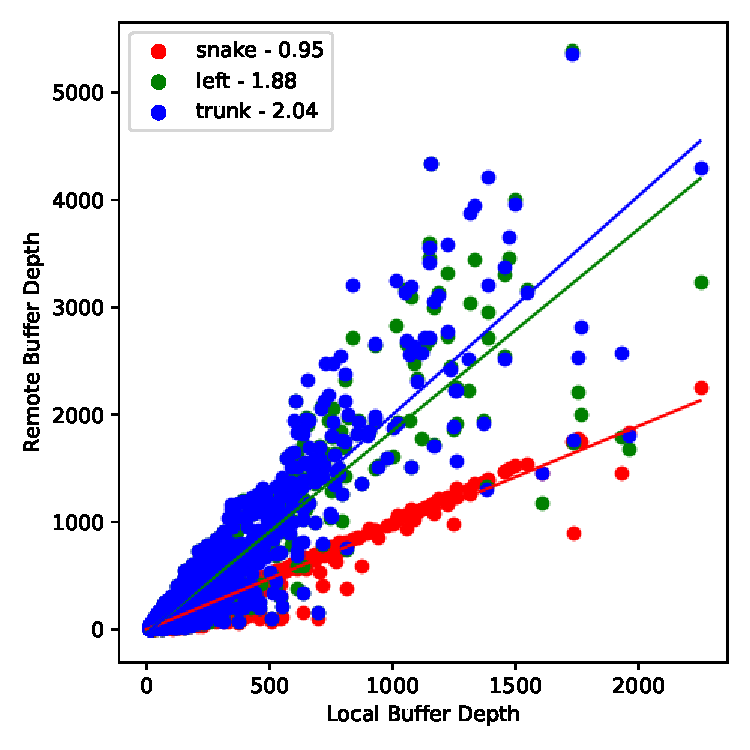
\includegraphics[width=\textwidth]{./images/mp60_16_slow_route_fits.pdf}
      \caption[]%
      {\small 16 Sized Tile}    
  \end{subfigure}
  \hfill
  \begin{subfigure}[b]{0.475\textwidth}  
      \centering 
      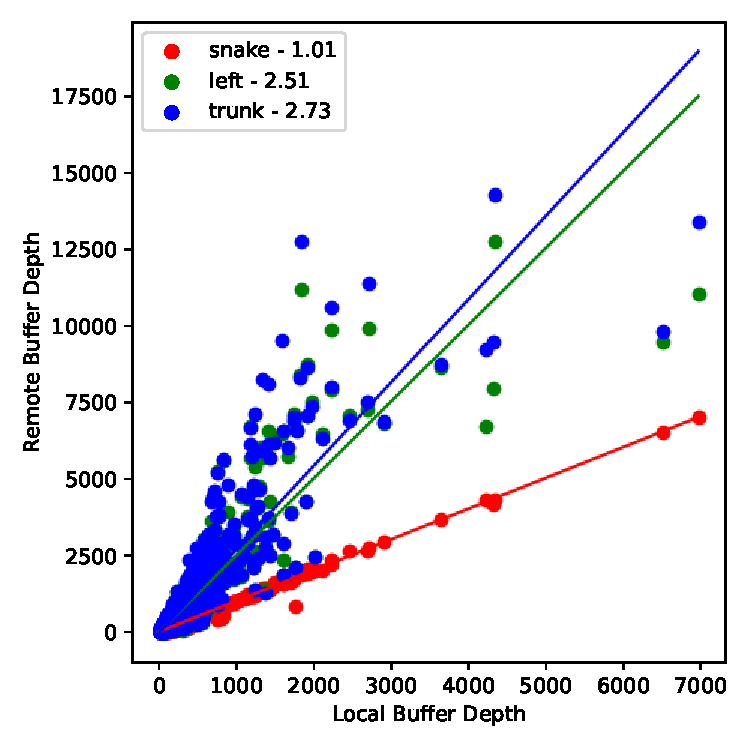
\includegraphics[width=\textwidth]{./images/mp60_64_slow_route_fits.pdf}
      \caption[]%
      {\small 64 Sized tile}    
  \end{subfigure}
  \vskip\baselineskip
  \begin{subfigure}[b]{0.475\textwidth}   
      \centering 
      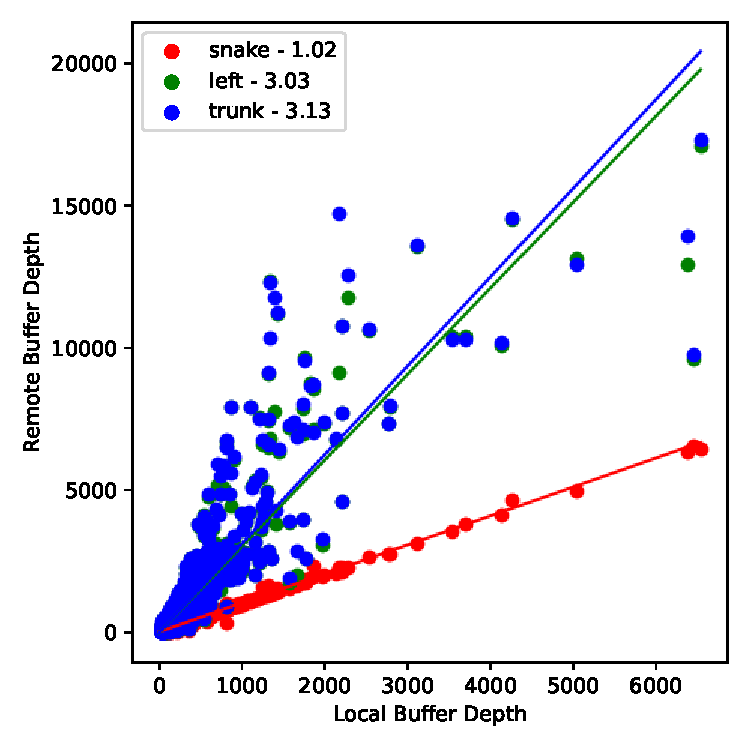
\includegraphics[width=\textwidth]{./images/mp60_140_slow_route_fits.pdf}
      \caption[]%
      {\small 140 Sized tile}    
  \end{subfigure}
  \hfill
  \begin{subfigure}[b]{0.475\textwidth}   
      \centering 
      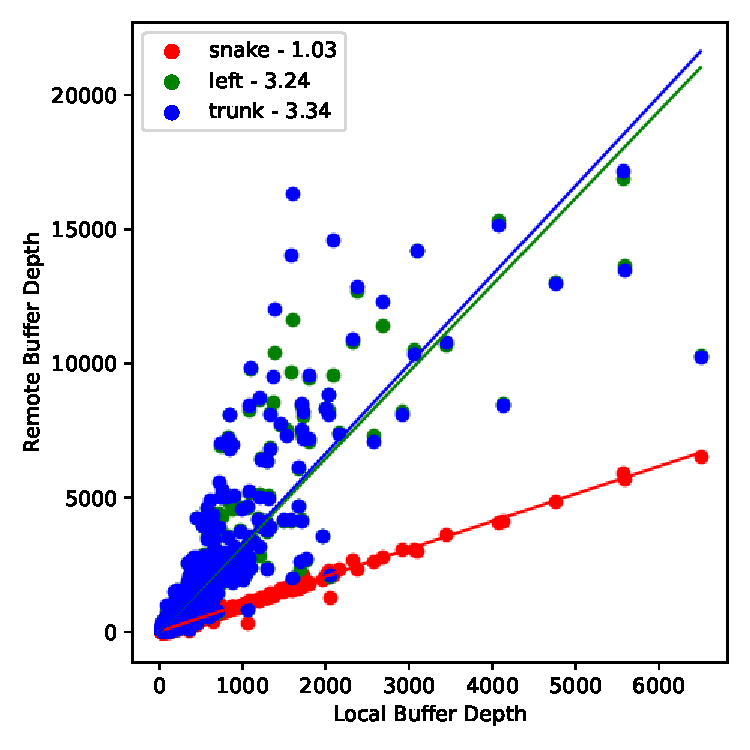
\includegraphics[width=\textwidth]{./images/mp60_256_slow_route_fits.pdf}
      \caption[]%
      {\small 256 Sized Tile}    
  \end{subfigure}
  \caption[ Information on the 4 by 4 tile. ]
  {\small all of the data } 
  \label{fig:compare_slow_plots_for_digital_sim_slow}
\end{figure*}


%%% 4x4 Example Digital simulation results
\begin{figure*}
  \centering
  \begin{subfigure}[b]{0.475\textwidth}
      \centering
      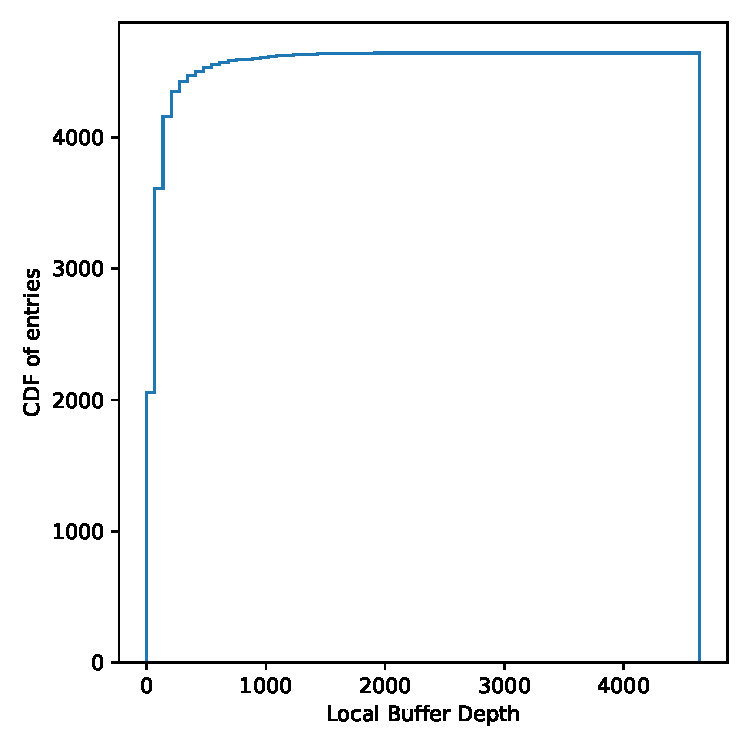
\includegraphics[width=\textwidth]{./images/mp60_16_fast_local_stack.pdf}
      \caption[Network2]%
      {{\small Network 1}}    
  \end{subfigure}
  \hfill
  \begin{subfigure}[b]{0.475\textwidth}  
      \centering 
      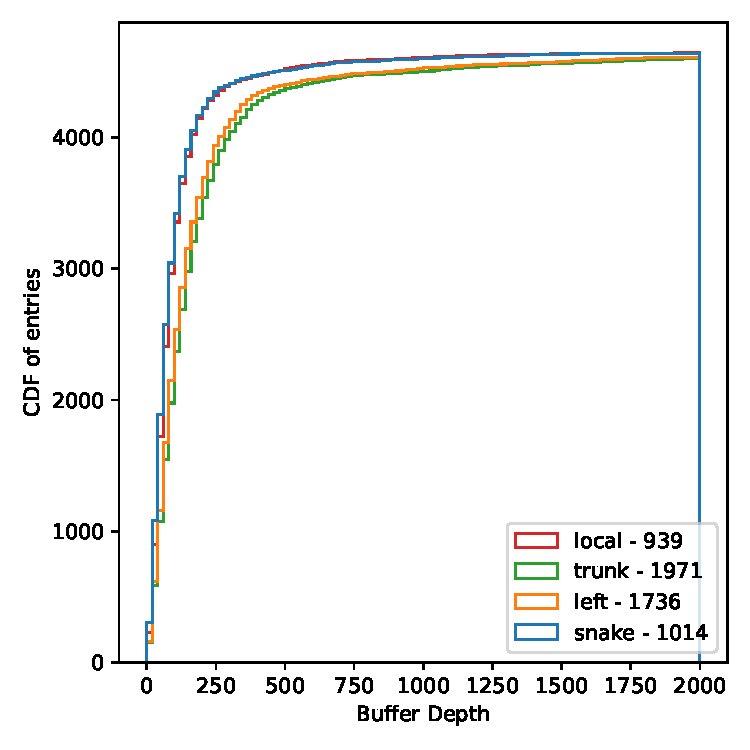
\includegraphics[width=\textwidth]{./images/mp60_16_fast_remote_stack.pdf}
      \caption[]%
      {{\small remote stack}}    
  \end{subfigure}
  \vskip\baselineskip
  \begin{subfigure}[b]{0.475\textwidth}   
      \centering 
      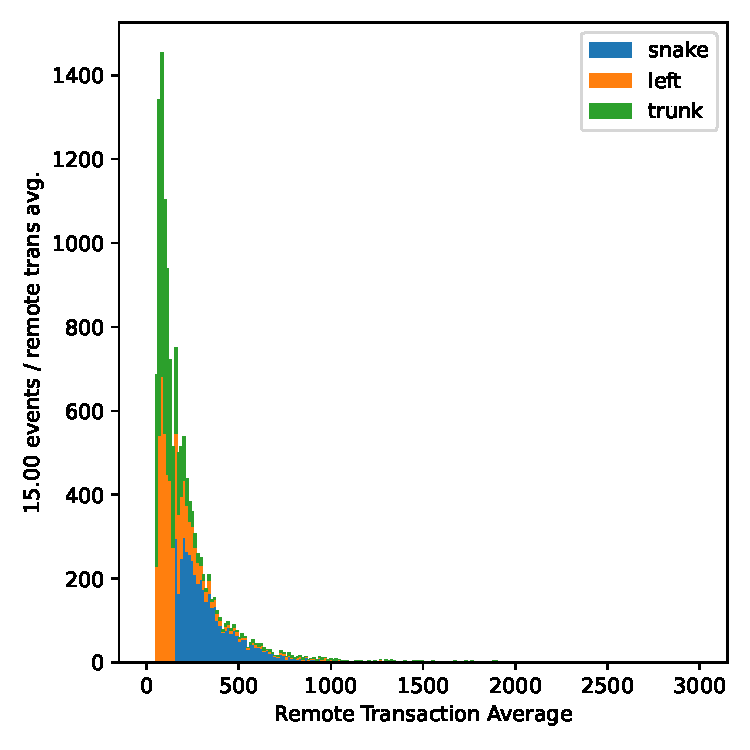
\includegraphics[width=\textwidth]{./images/mp60_16_fast_remote_transactions.pdf}
      \caption[]%
      {{\small transact}}    
  \end{subfigure}
  \hfill
  \begin{subfigure}[b]{0.475\textwidth}   
      \centering 
      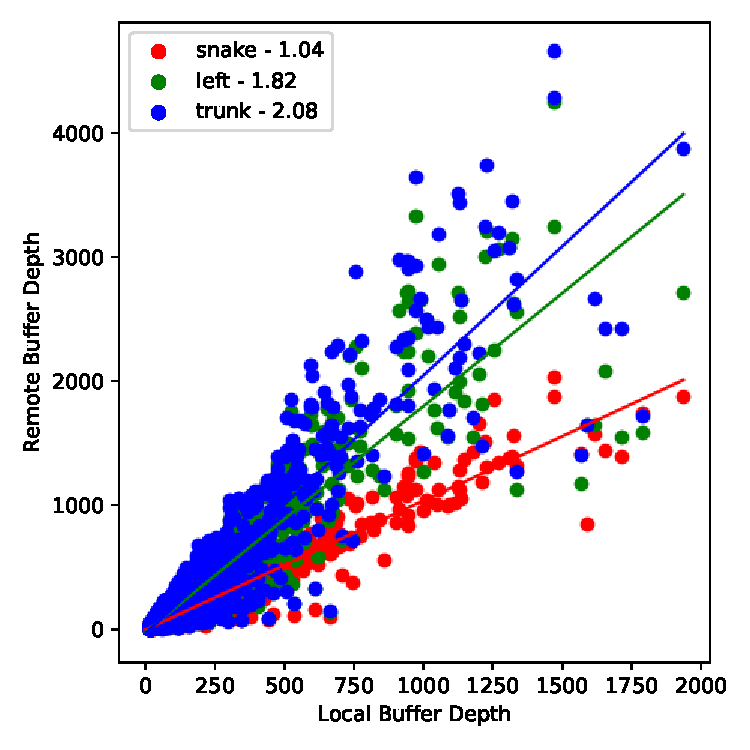
\includegraphics[width=\textwidth]{./images/mp60_16_fast_route_fits.pdf}
      \caption[]%
      {{\small route fits}}    
  \end{subfigure}
  \caption[ Information on the 4 by 4 tile. ]
  {\small example plots for a 4 $\times$ 4 tile. } 
  \label{fig:mp60_plots_for_digital_sim}
\end{figure*}

%%% Example of Digital Simulation Results for 16x16 tile
\begin{figure*}
  \centering
  \begin{subfigure}[b]{0.475\textwidth}
      \centering
      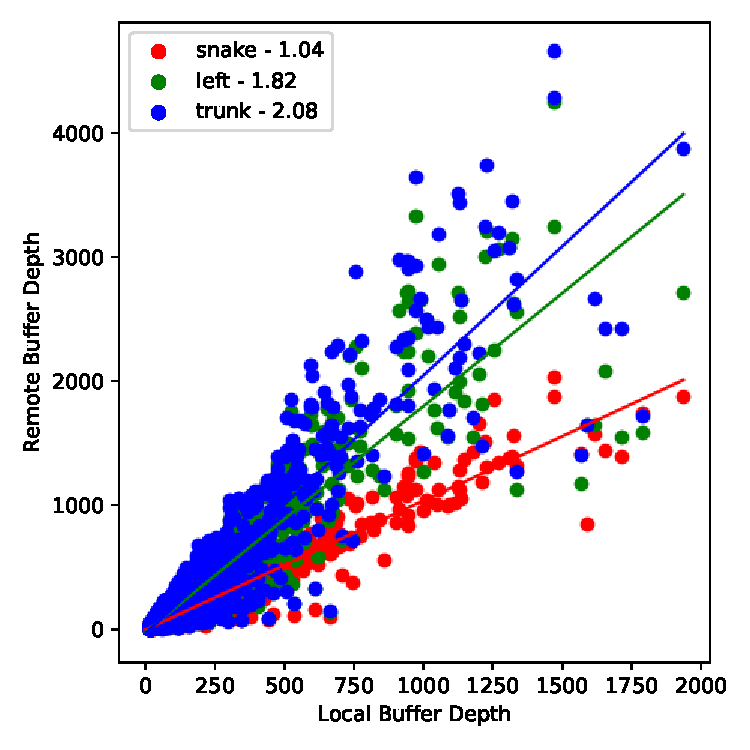
\includegraphics[width=\textwidth]{./images/mp60_16_fast_route_fits.pdf}
      \caption[]%
      {\small 16 Sized Tile}    
  \end{subfigure}
  \hfill
  \begin{subfigure}[b]{0.475\textwidth}  
      \centering 
      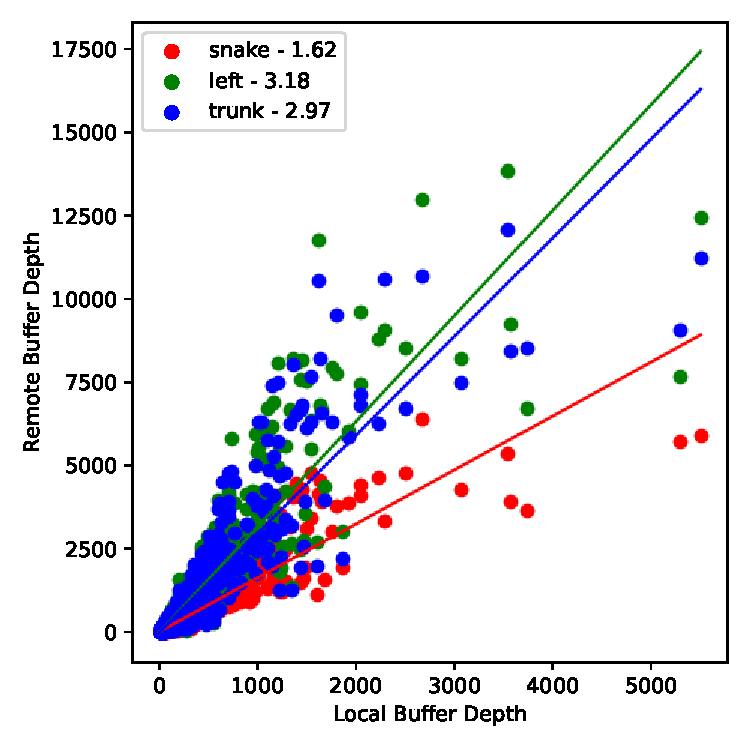
\includegraphics[width=\textwidth]{./images/mp60_64_fast_route_fits.pdf}
      \caption[]%
      {\small 64 Sized tile}    
  \end{subfigure}
  \vskip\baselineskip
  \begin{subfigure}[b]{0.475\textwidth}   
      \centering 
      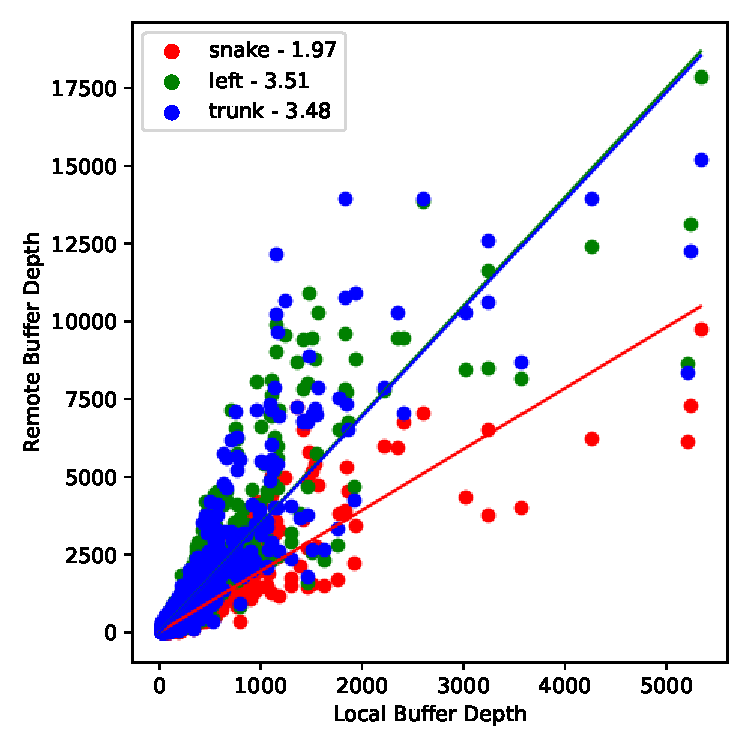
\includegraphics[width=\textwidth]{./images/mp60_140_fast_route_fits.pdf}
      \caption[]%
      {\small 140 Sized tile}    
  \end{subfigure}
  \hfill
  \begin{subfigure}[b]{0.475\textwidth}   
      \centering 
      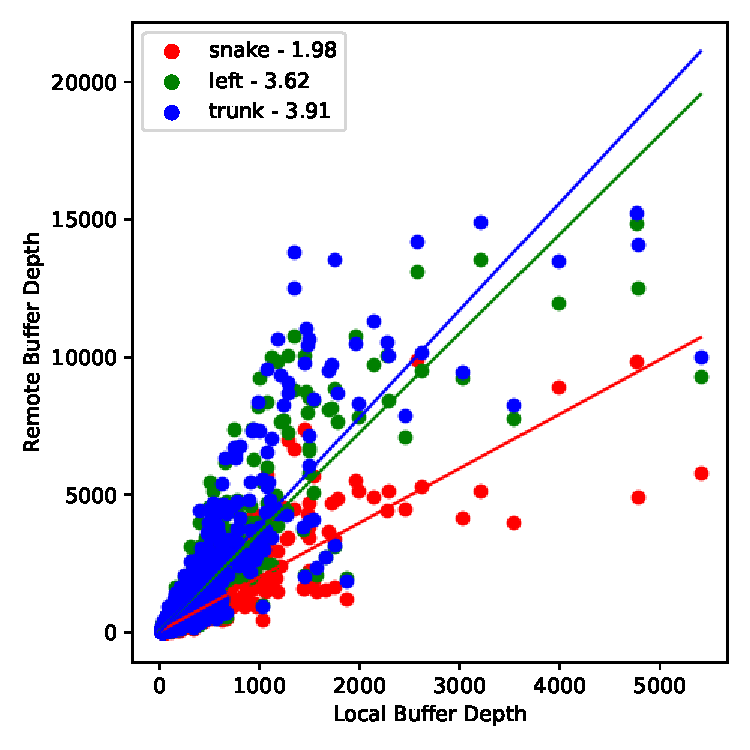
\includegraphics[width=\textwidth]{./images/mp60_256_fast_route_fits.pdf}
      \caption[]%
      {\small 256 Sized Tile}    
  \end{subfigure}
  \caption[ Information on the 16 by 16 tile. ]
  {\small 16 $\times$ 16 tile of results} 
  \label{fig:compare_fast_plots_for_digital_sim_fast}
\end{figure*}

%% table information
\begin{table}
	\begin{center}
		\begin{tabular}{|c|c|c|c|c|c|}
			\hline
			Freq. & Tile Size & Mean Local Hits & Snake & Left & Trunk \\
			\hline
			5\% & 16 & 48.250 & 423.293 & 166.403 & 138.380 \\
			\hline
			0.5\% & 16 & 51.846 & 449.861 & 177.357 & 147.346 \\
			\hline
			5\% & 64 & 34.129 & 1332.440 & 286.929 & 227.595 \\
			\hline
			0.5\% & 64 & 36.268 & 1400.794 & 301.775 & 239.087 \\
			\hline
			5\% & 140 & 26.521 & 2298.912 & 355.037 & 262.448 \\
			\hline
			0.5\% & 140 & 28.173 & 2416.778 & 373.173 & 275.614 \\
			\hline
			5\% & 256 & 24.343 & 4020.649 & 465.629 & 354.405 \\
			\hline
			0.5\% & 256 & 25.752 & 4209.196 & 487.090 & 370.695 \\
			\hline
		\end{tabular}
	\end{center}
	\caption{Transaction summary data is shown.
	The mean local hits column indicates the mean average of resets injected into the ASICs within the tile from an electron neutrino events.
	The Snake, Left, and Trunk, columns indicate the mean number of remote packet transactions which occured during the full 10 second simulation run.
	As expected, the amount of packet transactions in the snake routing scales with the tile size, whereas the Left and Trunk routings do not.
	The frequency distribution of the tiles does not affect the total number of transactions in the simulated event.
	These results can be used to indicate the amount of power and active time required for a tile to fully readout an electron neutrino event. 
	For example, if a tile size of 256 with a snake routing takes 4020 packets on average to digitize the event, then there are a total of slightly more than one million packets sent.
	If the amount of power used during single packet transaction is known, this ratio could be used to estimate the dissipated power during the back-end readout. 
	}
	\label{tab:transact}
\end{table}

%% table information
\begin{table}
	\begin{center}
		\begin{tabular}{|c|c|c|l|r|l|r|l|r|}
			\hline
			Freq. & Tile Size & Local Hits & 95-S & 99-S & 95-L & 99-L & 95-T & 99-T \\
			\hline
			5\% & 16 & 939 & 320 & 1014 & 535 & 1736 & 607 & 1971 \\
			\hline
			0.5\% & 16 & 1014 & 322 & 975 & 603 & 1949 & 652 & 2125 \\
			\hline
			5\% & 64 & 1200 & 598 & 2191 & 1098 & 4394 & 975 & 4295 \\
			\hline
			0.5\% & 64 & 1307 & 403 & 1328 & 970 & 4298 & 974 & 4521 \\
			\hline
			5\% & 140 & 1182 & 852 & 3486 & 1455 & 6558 & 1343 & 6309 \\
			\hline
			0.5\% & 140 & 1393 & 440 & 1464 & 1327 & 6616 & 1382 & 6757 \\
			\hline
			5\% & 256 & 1456 & 1039 & 3637 & 2026 & 7679 & 2008 & 8250 \\
			\hline
			0.5\% & 256 & 1670 & 527 & 1668 & 1773 & 7460 & 1784 & 7368 \\
			\hline
		\end{tabular}
	\end{center}
	\caption{Buffer Data}
	\label{tab:buffers}
\end{table}

%% table information
\begin{table}
	\begin{center}
		\begin{tabular}{|c c|c|c|c|c|}
			\hline
			Tile Size & Frequency & Snake & Left & Trunk & Push \\
			\hline
			16 & 0.5\% & 0.948 & 1.879 & 2.039 & 0.979 \\
			& 5\% & 1.041 & 1.823 & 2.082 & 1.031 \\
			\hline
			64 & 0.5\% & 1.006 & 2.514 & 2.727 & 0.999 \\
			& 5\% & 1.623 & 3.176 & 2.969 & 1.11 \\
			\hline
			140 & 0.5\% & 1.021 & 3.033 & 3.131 & na \\
			& 5\% & 1.966 & 3.506 & 3.481 & na \\
			\hline
			256 & 0.5\% & 1.027 & 3.243 & 3.336 & na \\
			& 5\% & 1.981 & 3.616 & 3.913 & na \\
			\hline
		\end{tabular}
	\end{center}
	\caption{Transaction fit summary results.
	The values shown from the fits indicate the linear fit to the results to predict the relationship between the local and remote FIFO depth requirements.
	Push fit data is not available for larger tiles (140 and 256) due to simulation time constraints.
	}
	\label{tab:fit}
\end{table}

\section{Summary and Further Studies}~\label{sec:further_studies}